% Template created by Karol Kozioł (www.karol-koziol.net) for ShareLaTeX

\documentclass[a4paper,9pt]{extarticle}
\usepackage[utf8]{inputenc}
\usepackage[T1]{fontenc}
\usepackage{graphicx}
\usepackage{xcolor}
\usepackage{tikz}
\usepackage[export]{adjustbox}

\usepackage{amsmath,amssymb,textcomp}
\usepackage{mathtools}
\usepackage{fixmath}
\usepackage[parfill]{parskip}
\usepackage{enumitem}
\everymath{\displaystyle}

\usepackage{times}
\renewcommand\familydefault{\sfdefault}
\usepackage{tgheros}
\usepackage[defaultmono,scale=0.85]{droidsansmono}
\usepackage{multicol}
\setlength{\columnseprule}{0pt}
\setlength{\columnsep}{20.0pt}


\usepackage{geometry}
\geometry{
a4paper,
total={210mm,297mm},
left=10mm,right=10mm,top=10mm,bottom=15mm}

\linespread{1.3}


% custom title
\makeatletter
\renewcommand*{\maketitle}{%
\noindent
\begin{minipage}{0.462\textwidth}
\begin{tikzpicture}
\node[rectangle,rounded corners=6pt,inner sep=10pt,fill=blue!0!white,text width= 0.95\textwidth] {\color{black}\Huge \textsf{\@title}};
\end{tikzpicture}
\end{minipage}
\hfill
\begin{minipage}{0.25\textwidth}
\begin{center}
\includegraphics[width=0.25\columnwidth]{IN_black.png}
\label{fig:HSRT}
\end{center}
\end{minipage}
\begin{minipage}{0.25\textwidth}
\begin{center}
\includegraphics[width=0.4\columnwidth]{TUM_blue.png}
\label{fig:TEC}
\end{center}
\end{minipage}
\bigskip %\bigskip
}%
\makeatother

% custom section
\usepackage[explicit]{titlesec}
\newcommand*\sectionlabel{}
\titleformat{\section}[runin]
  {\gdef\sectionlabel{}
   \normalfont\sffamily\Large\bfseries\scshape}
  {\gdef\sectionlabel{\thesection\ }}{0pt}
  {
\noindent
\begin{tikzpicture}
\node[rectangle,rounded corners=3pt,inner sep=4pt,fill=white!50!black,text width= 1.0\columnwidth] {\color{white}\sectionlabel#1};
\end{tikzpicture}
  }
\titlespacing\section{0pt}{15pt}{10pt}

%creative commons license logos
\usepackage{ccicons}

% custom footer
\usepackage{fancyhdr}
\makeatletter
\pagestyle{fancy}
\fancyhead{}
\fancyfoot[C]{\footnotesize \ccbysa\ ~ \@date\ ~ \@author}
\renewcommand{\headrulewidth}{0pt}
\renewcommand{\footrulewidth}{0pt}
\makeatother

%%%%%%%%%%%%%%%%%%%%%%%%%%%%%%%%%%%%%%%%%%%%%%%%%%%%%%%%
% -------Für ToDo-Notes---------------------------------
%%%%%%%%%%%%%%%%%%%%%%%%%%%%%%%%%%%%%%%%%%%%%%%%%%%%%%%%
\usepackage[color=red, shadow]{todonotes} % ", disable" deaktiviert ToDo-Notes
%Vereinfachtes "Inline-Todo"
\newcommand{\td}[1]{{\todo[inline]{#1}}}
\newcommand{\tdu}[1]{{\todo[inline, color=green!40]{#1}}}

\usepackage{url}
\graphicspath{{images/}}

\usepackage[
	colorlinks=true,
	urlcolor=blue,
	linkcolor=black
]{hyperref}

\title{Robot Motion Planning}
\author{\url{https://github.com/MichaelGrupp/RobotMotionPlanning_summary} \\ TU München - Fakultät für Informatik - Robotics, Cognition, Intelligence}
\date{\the\year}


\begin{document}

\maketitle

\begin{multicols*}{2}  %2 columns, uncomment \end{multicols*} too if you want single column


\section{Introduction}
The main problem is to find a path from one position or configuration to another, without colliding with the environment. Planning algorithms can be rated regarding different aspects.\par

Performance metrics for path planning algorithms:
\setlist{nosep}
\begin{itemize}
	\item path length
	\item execution speed
	\item planning time
	\item safety (distance to obstacles)
	\item robustness to disturbances
	\item probability of success
\end{itemize}
\vspace{2.5mm}
To avoid long calculations in online processes, often an offline
pre-processing is done and a road-map is calculated. When
the manipulator is high-complex it is not possible to calculate
the road-map beforehand and thus probabilistic approaches are
used. Those perform sampling and create the road-maps with
uncertain data.

\section{Configuration Space}
\subsection{Basics}
\textbf{Workspace:} Reachable space of the end-effector. \\
\textbf{Task space:} Corresponds to the space where the robot's task can be naturally expressed. \\
\textbf{Configuration:} The smallest number of real-valued coordinates to fully describe configurations of a robot. For example, a mobile robot moves in directions $x,y$ and can turn its yaw heading $\theta$ - a configuration of this robot could be $\mathbold{c} = (1,3,30^\circ)^\mathrm{T}$. \\
\textbf{Configuration space (\textit{C-space}):} The space of all possible configurations, that a robot can have in a certain workspace. \\
\textbf{Dimension of the C-space/DoF:} Minimum number of parameters needed to specify the configuration. Because there can also be angles in the topology of the C-space, it is usually not a Cartesian space (e.g. $2\pi = 4\pi$, cyclic repetition along angle axis). \\
\textbf{Common robot models:} Single points, single rigid bodies and multiple rigid bodies with joints. \\
\textbf{Non-holonomic robot:} Robot, that cannot move freely on the
configuration space manifold because it is constrained in some way. For example, a car cannot drive sideways. \\
\textbf{Path:} Continuous curve in configuration space $C$ connecting two configurations $q$ and $q'$:
$\tau: s \in [0,1] \rightarrow \tau(s) \in C$ s.t. $\tau(0) = q$ and $\tau(1) = q'$\\
\textbf{Trajectory:} A trajectory is a path parametrized by time:
$\tau: t \in [0, T] \rightarrow \tau(t) \in C$.
Possible constraints: Smoothness, minimum length, minimum time, ...

\subsection{Calculate DoF}
\textbf{Calculate DoF of a single body:}
DoF = total DoF of 3 fixed points - number of constraints (of the 3 fixed points, e.g. distances between points). \\
\textit{Alternative:} Find DoF of one point, go the next one and apply constraints, go to the third point and apply constraints. \par

\textbf{Calculate DoF for general robots:}
\begin{itemize}
	\item Open chains: Add the DoF of each joint
	\item Closed chains:\\
	$DoF = N(k-1) - \sum_{i=1}^{n} (N-f_i) = N(k-n-1) + \sum_{i=1}^{n} f_i$ \\
	– $N=6$ for 3D, $N=3$ for 2D\\
	– $k =$ number of links (including ground link)\\
	– $n =$ number of joints\\
	– $f_i =$ DoF of the $i^{th}$ joint
\end{itemize}

\subsection{Parametrizations of configurations}
Configuration: $\mathbold{q}=(position, orientation)=(x,y,z,\cdot)$.
There exist different ways how to parametrize orientations:
\begin{itemize}
	\item \textbf{Parametrization of orientations by rotation matrix:}\\
		$R=
		\begin{psmallmatrix}
			r_{11} & r_{12} & r_{13}\\
			r_{21} & r_{22} & r_{23}\\
			r_{31} & r_{32} & r_{33}
		\end{psmallmatrix}$
		with $\det(R)=1$ and $R^T R=I$ (or $R R^T=I$) \\
		Columns of $R$: Coordinate axes of new coordinate System
	\item \textbf{Parametrization of orientations by Euler angles:}\\
	Different sequences of rotation axes exist, e.g. "Roll, Pitch, Yaw" around $x$, $y$ and $z$:
	\begin{align*}
		R_{xyz}(\alpha, \beta, \gamma) &= R_z(\gamma)R_y(\beta)R_x(\alpha)=\\
		&=
		\begin{psmallmatrix}
			c\gamma & -s\gamma & 0\\
			s\gamma & c\gamma & 0\\
			0 & 0 & 1
		\end{psmallmatrix}
		\begin{psmallmatrix}
			c\beta & 0 & s\beta\\
			0 & 1 & 0\\
			-s\beta & 0 & c\beta
		\end{psmallmatrix}
		\begin{psmallmatrix}
			1 & 0 & 0\\
			0 & c\alpha & -s\alpha\\
			0 & s\alpha & c\alpha
		\end{psmallmatrix}
	\end{align*}
	Problem: Singularities
	\item \textbf{Parametrization of orientations by unit quaternions:}\\
	$\mathbold{u} = (cos(\theta/2), n_x sin(\theta/2), n_y sin(\theta/2), n_z sin(\theta/2))$\\
	with $\lVert \mathbold{n} \rVert = 1$ ($\mathbold{n}$: rotation vector, $\theta$: rotation angle)\\
	Advantages: Compact, no singularities, natural orientation representation
\end{itemize}

\subsection{Configuration space}
\textbf{C-space $C$:} $F \cup C_{obs}$\\
\textbf{Free space $F$:} All collision-free configurations (open subset of $C$).\\
\textbf{Obstacle space $C_{obs}$:} Set of configurations which lead to a collision with workspace obstacles (closed subset of $C$).\\
\textbf{Semi-free space:} A configuration $q$ is semi-free if the robot placed $q$ touches the boundary, but not the interior of obstacles. $F \, \cup \, \partial C_{obs}$\\
\textbf{Determine free space:} Discretize the configuration space and check for each grid cell if the corresponding configuration leads to a collision in the workspace (brute-force approach).

\subsection{Point representation}
In order to determine the C-space / free space of configurations, a point representation can be useful. For example, if we have a circular robot with radius $r$ and some obstacles in the workspace, the robot can be reduced to a point if the obstacle boundaries are "blown up" by the radius of the robot. In other words, to get a smaller representation of the robot without changing the properties of the workspace, the obstacles have to get bigger. 
$\Rightarrow$ Minkowski sum algorithm

\begin{center}
\includegraphics[width=0.3\columnwidth]{pointrep}
\end{center}

\subsection{Collision Detection}
Create a hull (circle, rectangle, convex hull, …) around an object and
perform a collision check. Circle: 1 distance calculation. Rectangle (axis aligned): 4 distance calculations.\\
Circle approach: Start with one big circle, perform check: if collision, split circle into smaller circles and repeat until minimum radius is reached, else no collision.

\begin{center}
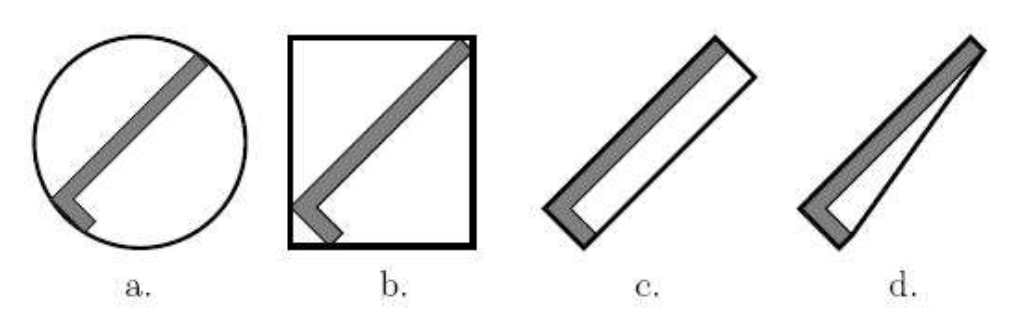
\includegraphics[width=\columnwidth]{collision_hull.png}
\end{center}

\section{Bug Algorithms}
Bug algorithms are simple strategies that use local knowledge (e.g. from sensor input) instead of global knowledge.\par

\textbf{Assumptions:}
\begin{itemize}
	\item Robot is a point in a plane.
	\item Contact sensor to detect obstacle boundaries.
\end{itemize}

\textbf{Basic idea:} Move on a straight line towards goal and follow the boundaries around obstacles.

\subsection{Bug 0}
\begin{enumerate}
	\item Head towards the goal.
	\item When hit point set, follow the wall until you can move towards goal again (leave point).
	\item Continue from 1.
\end{enumerate}
Fails for certain obstacle shapes! (e.g. spiral)

\begin{center}
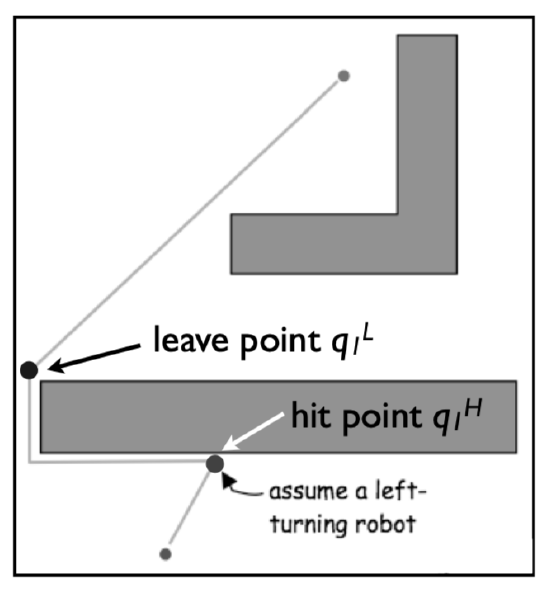
\includegraphics[width=0.4\columnwidth]{bug0.png}
\end{center}

\subsection{Bug 1}
\begin{enumerate}
	\item Move towards goal on the \textit{m-line} connecting $q_{start}$ and $q_{goal}$.
	\item If an obstacle is detected at a hit-point $q^H_i$, move left (or right) along its boundary until you return to $q^H_i$ again.
	\item While circumnavigating the obstacle, calculate and save the distance to the goal at any coordinate.
	\item Determine the closest point to the goal on the boundary and use it as a leave point $q^L_i$.
	\item From $q^L_i$, go straight to the goal again on the m-line $q^L_i$ and $q_{goal}$.
	\item If the line that connects $q^L_i$ and the goal intersects the current obstacle, then there is no path to the goal.
\end{enumerate}
\begin{center}
\includegraphics[width=0.6\columnwidth]{bug1.png}
\end{center}

\noindent \textit{Worst case:} $L_{Bug1} \leq d(q_{start}, q)+1.5\sum_{i=1}^{n} p_i$ with $p_i$ being the length of the contour of the $i$-th obstacle.\\
\textit{Best case:} $d(q_{start}, q)$.\\
\textit{Problems:} Fails when started inside of closed obstacles and possibly changed approach vector to the goal (problematic when grabbing objects).

\subsection{Bug 2}
The m-line of Bug 2 does not change and it connects $q_{start}$ and $q_{goal}$.
\begin{enumerate}
	\item Move towards goal on the \textit{m-line} connecting $q_{start}$ and $q_{goal}$.
	\item If an obstacle is detected at a hit-point $q^H_i$, move left (or right) along its boundary.
	\item If a point on the m-line is found and it is closer to the goal than $q^H_i$, use it as a leave point $q^L_i$.
	\item From $q^L_i$, go straight to the goal again on the m-line.
	\item If the robot re-encounters the original departure point $q^H_i$ from the m-line, then there is no path to the goal.
\end{enumerate}
\begin{center}
\includegraphics[width=0.7\columnwidth]{bug2.png}
\end{center}

\noindent Fails when started inside of closed obstacles. Problematic shapes: spirals. Worst case: $L_{Bug2} \leq d(q_{start}, q)+0.5\sum_{i=1}^{n} n_i p_i$ with $n_i$ being the number of times that the m-line hits the obstacle.

\subsection{Tangential Bug}
The robot is equipped with a (finite-range) radial distance sensor. If an obstacle is encountered within the range of the sensor, the robot changes its direction tangentially to the border of the obstacle.

\begin{center}
	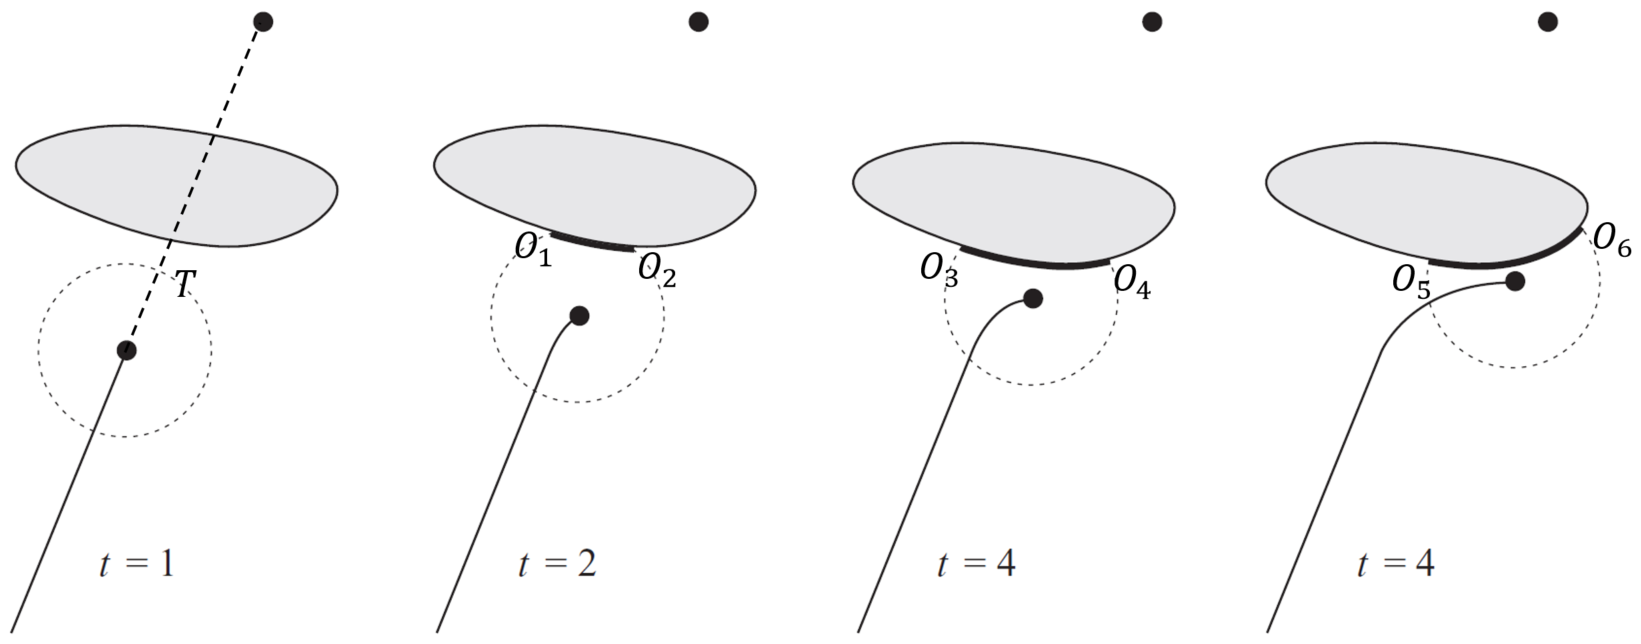
\includegraphics[width=\columnwidth]{tangential_bug.png}
\end{center}

\noindent Essentially, the bug algorithms have two behaviors: Drive toward a point and follow an obstacle.

\begin{center}
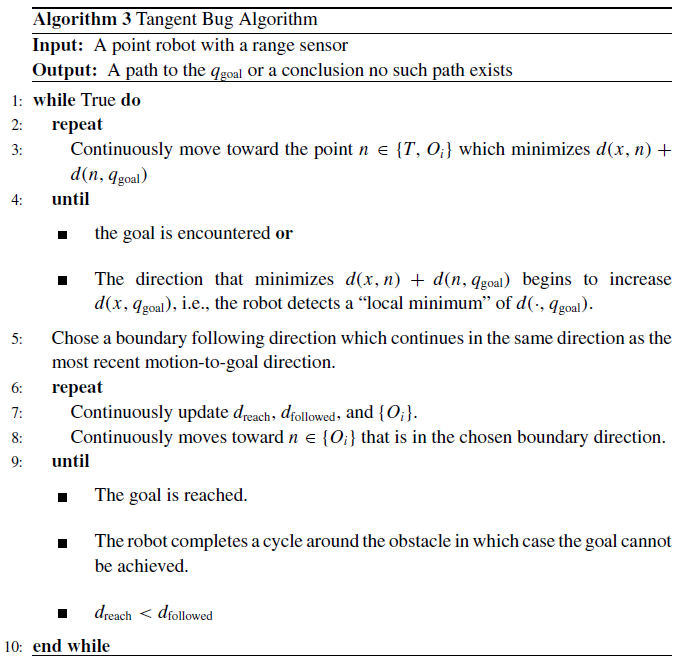
\includegraphics[width=\columnwidth]{tangential_bug_pseudocode.PNG}
\end{center}
$d_{\text{followed}}$ is the shortest distance between the boundary which had been sensed and the goal.
$d_{\text{reach}}$ is the distance between the goal and the closest point on the followed obstacle that is within line of sight of the robot.

\section{Planners}
In order to describe more complicated path planners, we need to be able to specify the position of the robot and the (C-)space it occupies.
Gradients work by changing the repulsive potential as a robot gets closer to an obstacle. The start point is given a medium gradient potential, the end point is given a low gradient potential, and the obstacles are given high gradient potentials.
All the robot needs to do is “roll down the hill.”

\subsection{Brushfire Planner}
The Brushfire Algorithm is a discrete version of the aforementioned gradient algorithm and involves the use of a grid to determine the potential of cells.
It starts the fire at all boundaries of obstacles and overall boundary and iterates through the grid.
”2” for cells neighboring an obstacle and so on.
When two weights meet, same distance to obstacles is achieved (important for Voronoi).

\subsection{Wave-Front Planner}
Variation of the Brushfire algorithm. Using a grid it assigns a “1” to each cell that has an obstacle (or part of an obstacle).
The start point is labeled “2” and the “wave” propagates from that point. Each adjacent cell, if empty, is given an incrementally higher number until all the cells have a number.
If the goal has a number in its cell, the goal is reachable in that many moves minus one.
The algorithm can also start from the goal towards the start.\\
\textit{Benefit:} Avoids the local minima problem by planning one step at a time on a grid.

\section{Classical path planning}
Using offline pre-processing and exact environment knowledge in order to do the path planning beforehand and save online performance, we distinguish:
\begin{itemize}
	\item Roadmaps
	\item Cell decomposition
	\item Potential field
\end{itemize}

\subsection{Roadmaps (with exact knowledge)}
\textit{Idea:} Represent the connectivity of the free space in a network of 1D curves.\par
Using this network, paths can be calculated using graph-search algorithms, for example.\\ \textit{Advantage:} Roadmap has to be constructed once if the topology of the workspace (i.e. obstacle positions) does not change.\\
\textit{Disadvantage:} Roadmaps can be not very efficient in dynamic environments.

\subsubsection{Visibility Graph}
The visibility graph applies to 2D spaces with polygonal obstacles.\\
Nodes: $q_{init}$ (start) and $q_{goal}$ (goal) and obstacle vertices.\\
Edges: Two nodes are connected with an edge if the connecting line is an obstacle edge or does not intersect with an obstacle.
Time $O(n^3)$, space $O(n^2)$.

\begin{center}
\includegraphics[width=0.6\columnwidth]{visGraph}
\end{center}

\noindent The visibility graph can contain useless edges.
This can be resolved by constructing the reduced visibility graph, where only edges are kept that are separating or supporting lines between two obstacles (or lines on the border of obstacles). 

\begin{center}
\includegraphics[width=0.6\columnwidth]{visGraph2}
\end{center}

\subsubsection{Voronoi Diagram}
The goal of the Voronoi diagram is to find paths that maximize the distance to the obstacles. Therefore, the roadmap lines can be curved.\\
Time $O(n \log n)$, space $O(n)$.

\begin{center}
\includegraphics[width=0.6\columnwidth]{voronoi}
\end{center}

\noindent To construct the Voronoi diagram, one can use the Brushfire algorithm, which calculates a distance map on a grid:
\begin{itemize}
	\item Grid initialization: free space = 0, obstacle space = 1
	\item For each point in the grid, it assigns the distance to the closest obstacle point.
	\item Every point, where the distance to two (or more) different obstacles is the same, lies on the Voronoi diagram.
\end{itemize}
$\rightarrow$ "Wavefront from obstacles, Voronoi diagram where two wavefronts meet."\\

\subsection{(Vertical) Cell Decomposition}
\textit{Idea:} Decompose the free space into simple cells and represent the connectivity of the free space $F$ by the adjacency graph of these cells (mostly in 2D).\par

It is called an exact cell decomposition if the union of all cells is exactly $F$, meaning there is no overlap between cells.
The shape of the cells can be triangles, trapezoids, ...

\subsubsection{Trapezoidal Decomposition}
Free space is decomposed into trapezoids and triangles. Then, the adjacency graph of the cells is calculated.\\
Time $O(n \log n)$, space $O(n)$.

\begin{center}
\includegraphics[width=0.7\columnwidth]{cell}
\end{center}

\noindent The planner searches the adjacency graph to determine the path of nodes.
Then the planner constructs the point to point path, one trapezoid at a time, by connecting the midpoints of the vertical extensions to the centroids of each trapezoid.
To connect the start and goal points, simply draw a straight line to the vertical extensions’ midpoints of the appropriate trapezoids.

\subsubsection{Boustrophedon Decomposition}
Points on the obstacles, from which a separating line can be drawn in the upper and lower direction are called critical points. Then, an exhaustive walk through the critical points is performed in order to obtain a connectivity graph.
\begin{center}
\includegraphics[width=\columnwidth]{boustro}
\end{center}

\subsection{Cell Decomposition in higher dimensions}
\subsubsection{The Halting Problem}
\textbf{Completeness:} A complete algorithm finds a path if one exists and reports no otherwise.\par
Is it possible to determine whether a program will stop or will it run forever?\\
Suppose an algorithm $H$ that can decide whether $X$ will halt.
By proof by contradiction, it can be shown that such an algorithm $H$ cannot exist.
Furthermore, it can be shown that not all planning algorithms are complete.\\
\textit{But:} Combinatorial algorithms (cell decomposition, visibility graphs \& Voronoi diagrams) are completed since they cover every single point in $C_{free}$. $\rightarrow$ Motivates the use of combinatorial algorithms of rhigher dimensions.

\subsubsection{Extension of vertical Cell Decomposition}
Extension of vertical CD to $n$ dimensions:
\begin{enumerate}
	\item Pick a dimension $x_i$
	\item Sweep the configuration space using a (n-1)-dimensional plane orthogonal to $x_i$. Stop when critical connectivity events happen. When such a change happens, a new (n-1)-dimensional slice is produced.
	\item Repeat for the (n-1)-dimensional slices
	\item Sweeping yields convex n-cells, (n-1)-cells, ... (with a n-cell being a n-dim. polytope sandwiched between (n-1)-dim. slices).
\end{enumerate}

\subsubsection{k-d tree}
Tree like data structure useful for finding points with certain properties. Construction:
\begin{enumerate}
	\item Pick dimension $i$, pick a point with coordinates $x$.
	\item Split the points based on $x_i$ (greater or less than).
	\item Repeat the above two steps recursively.
\end{enumerate}
\textit{Note:} $\text{depth} = \log n$ if balanced; construction takes $O(kn \log n)$ time.\\
Disadvantage: If the environment changes the k-d tree needs to be fully recomputed.

\subsection{Approximate Cell Decomposition}
\textit{Idea:} The free space $F$ is represented by a collection of non-overlapping cells whose union is contained in $F$.\\
Cells usually have simple, regular shapes. It facilitates the hierarchical space decomposition.
Examples are Quadtrees (2D) and Octrees (3D):
\begin{itemize}
	\item Splitting stops if node is empty or full (e.g. up to $95\%$).
	\item Advantage: If the environment changes only some nodes need to be recomputed (not the whole tree).
\end{itemize}
\begin{center}
	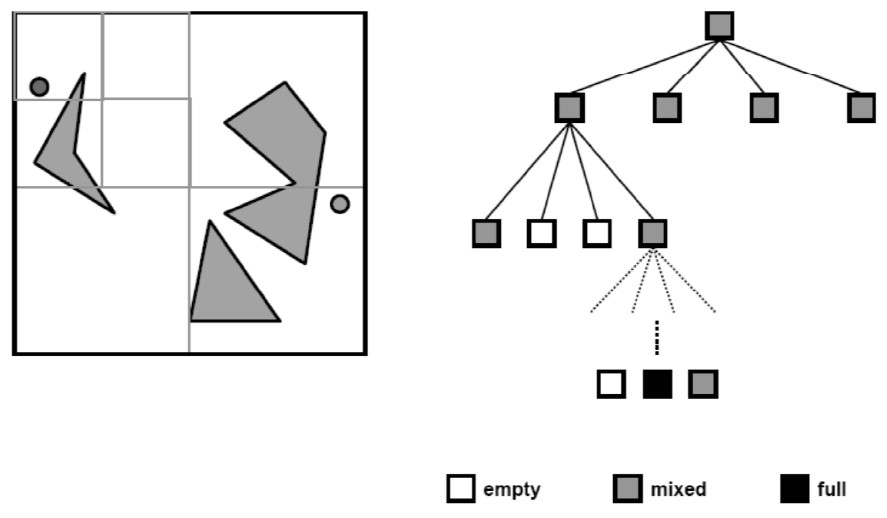
\includegraphics[width=0.85\columnwidth]{quadtree.jpg}
\end{center}

\subsection{Potential Field Method}
\textit{Idea}: Define a potential function over the free space that has a global minimum at the goal and follow the steepest descent of the potential function (gradient descent).\par
\noindent Obstacles are surrounded by a repulsive field and the goal location by an attractive field. Ideal potential field:
\begin{itemize}
	\item Global minimum at the goal.
	\item No local minima.
	\item Grows to infinity near obstacles.
	\item Is smooth.
\end{itemize}
\textit{Advantage:} Easy to compute.\\
\textit{Disadvantage:} Possible local minima (where robot gets stuck) and no consideration of dynamic constraints in their initial form (forces can be too high for the robot).

\begin{center}
	\includegraphics[width=0.6\columnwidth]{potential}
\end{center}

\noindent \textbf{\textit{Attractive component:}} A linear potential function results in a constant velocity (gradient) and thus an overshoot at the goal.
That is why a quadratic function is better suited since the minimum is reached with a velocity of 0.
Generally, it is combined with a linear function at a distance $d^*$ so that the gradient (which corresponds to the velocity) is not too large for the robot.

\begin{equation*}
	U_{att}(q) =
	\left\{\begin{matrix}
		\frac{1}{2}\zeta d^2(q,q_{goal}), & d(q,q_{goal}) \leq d^{*}_{goal} \\
		d^{*}_{goal}\zeta d(q,q_{goal}) - \frac{1}{2}\zeta (d^{*}_{goal})^2, & d(q,q_{goal}) > d^{*}_{goal} \\
	\end{matrix}\right.
\end{equation*}
\begin{equation*}
	\nabla U_{att}(q) =
	\left\{\begin{matrix}
		\zeta (q - q_{goal}), & d(q,q_{goal}) \leq d^{*}_{goal} \\
		\frac{d^{*}_{goal}\zeta(q - q_{goal})}{d(q - q_{goal})}, & d(q,q_{goal}) > d^{*}_{goal} \\
	\end{matrix}\right.
\end{equation*}

\noindent\textit{\textbf{Repulsive component:}} $Q^{*}$: Radius around obstacle where the repulsive force acts. $D(q)$: Distance to obstacle. 
\begin{equation*}
	U_{rep}(q) =
	\left\{\begin{matrix}
		\frac{1}{2}\eta \left (\frac{1}{D(q)} - \frac{1}{Q^*}\right )^2, & D(q) \leq Q^{*} \\
		0, & D(q) > Q^{*} \\
	\end{matrix}\right.
\end{equation*}
\begin{equation*}
	\nabla U_{rep}(q) =
	\left\{\begin{matrix}
		\eta \left (\frac{1}{Q^*} - \frac{1}{D(q)}\right ) \frac{1}{D^2(q)} \nabla D(q), & D(q) \leq Q^{*} \\
		0, & D(q) > Q^{*} \\
	\end{matrix}\right.
\end{equation*}

\section{Roadmapping with Random Sampling}
\textit{Problem with classical approaches:} Running time increases exponentially with the dimension of the C-Space. Modelling the free space becomes an arduous task.\par
Instead of looking at the whole space, sampling based methods are usually more efficient because they only require point-wise evaluations.
They are probabilistically complete (+), meaning the probability that they will produce a solution approaches 1 as more time is spent.
By reducing the map to samples, it will be easier to find a solution path since the computation effort is reduced and they can be applied to high-dimensional C-spaces (+).
However, they are not as robust as methods with full knowledge of the space and cannot determine if there is no solution to the path planning problem.\par

Sampling uniformly in 2D and 3D has to be correctly parametrized! Cases:
\begin{itemize}
	\item Unit line, square, cube: Pick a random number $r \in [0, 1]$
	for each dimension.
	\item Sample in interval $[a,b]$: $(b-a)r + a, \ r \in [0, 1]$.
	\item Angle: Pick angle $\theta$ uniformly at random from $[0, 2\pi]$.
	\item Rotations: Depends on the representation, in axis-angle notation the axis and the angle are sampled separately.
\end{itemize}


\subsection{Multi-Query}
A multiple query approach tries to capture the connectivity of the free space as good as possible with the goal to answer multiple, different queries for paths very fast.\\
Assumption: Static obstacles.

\subsubsection{PRM - Probabilistic Roadmaps}
\textbf{Basic steps for constructing PRMs:}
\begin{enumerate}
	\item Sample vertices (uniformly) and keep vertices that do not collide with obstacles (= milestones).
	\item Find neighbour vertices/milestones with
		\subitem k-nearest neighbour or
		\subitem neighbours within a specified radius.
	\item Connect neighbouring vertices with edges (lines) (and check for collisions on connecting line using e.g. discretized line search).
	\item Add vertices and edges until roadmap is dense enough.
\end{enumerate}
\begin{center}
\includegraphics[width=\columnwidth]{PRM}
\end{center}
\textbf{Query processing:}
\begin{enumerate}
	\item Connect $\mathbold{q}_{start}$ and $\mathbold{q}_{goal}$ with the graph (check for collisions on connecting line).
	\item Search a path from $\mathbold{q}_{start}$ to $\mathbold{q}_{goal}$ in the graph.
\end{enumerate}
\textbf{Drawback 1:} PRMs don't perform well when there are narrow passages ($\rightarrow$ you probably won't end up with a fully connected graph).\\
\textbf{Solution 1:} \textit{Expansion}
\begin{itemize}
	\item Further sampling ($\rightarrow$ increase number of nodes).
	\item Resampling with a random walk (when an obstacle is hit, continue in a random direction until a maximum length $L$ is reached).
	\item Bridge Sampling which focuses on generating samples in narrow passages.
	\item OBPRM.
\end{itemize}

\textbf{Drawback 2:} Many abrupt velocity changes due to the typical zick-zack paths.\\
\textbf{Solution 2:} Smooth the resulting path.\par

\textbf{Advantages of PRMs:}
\begin{itemize}
	\item Probabilistically complete.
	\item Apply easily to high-dimensional C-space.
	\item Fast queries (with enough preprocessing).
\end{itemize}

\textbf{Homotopic paths:} Two paths with the same endpoints are homotopic if one can be continuously deformed into the other.
A homotopic class of paths contain all paths that are homotopic to one another.
Homotopy ensures that after the path correction, the space topology gets visited from the same side as originally planned.
(If during the merging process the path goes through an object, it is not considered homotopic.)

\subsubsection{OBPRM - Obstacle-Based PRM}
Obstacle-based PRMs are constructed by sampling only close to obstacles.\par

Basic idea (for workspace obstacle $S$):
\begin{enumerate}
	\item Find a point in $S$'s C-obstacle (robot placement colliding with $S$).
	\item Select a random direction in C-space.
	\item Find a free point in that direction.
	\item Find boundary point between them using binary search (collision checks).
\end{enumerate}

\begin{center}
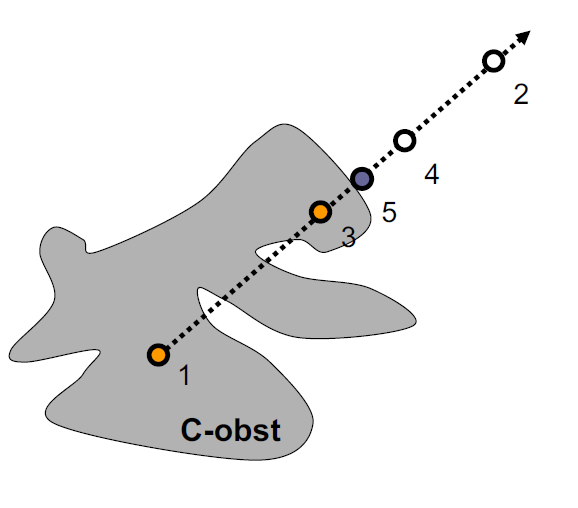
\includegraphics[width=0.5\columnwidth]{OBPRM_2}
\end{center}

\subsection{Single-Query PRM}
Single query planners try to solve a single query as fast as possible, without trying to cover the whole free space.\par

\textbf{Idea:} Grow two trees from \textit{Start} and \textit{Goal} configurations.
Randomly sample nodes around existing nodes.
Connect a node in the tree rooted at \textit{Start} to a node in the tree rooted at \textit{Goal}. $\rightarrow$ Expansion + Connection.\par

\textbf{Expansion + Connection:}
\begin{enumerate}
	\item Expand trees from \textit{Start} and \textit{Goal}.
	\item Pick a node $x$ with probability $1/w(x)$ ($w(x)$: number of nodes within certain radius, including node $x$)
	\item Randomly sample $k$ points ($y_1, ..., y_k$) around $x$.
	\item Add sample $y_i$ with weight $w(y_i)$	and probability $1/w(y_i)$ to the tree if
	\begin{itemize}
		\item $\frac{1}{w(y_i)} > \frac{1}{w(x)} \Leftrightarrow w(y_i) < w(x)$.
		\item $y_i$ is collision free.
		\item $y_i$ can see $x$.
	\end{itemize}
	\item If a pair of nodes from start tree and goal tree are close and can see each other, then connect them and terminate.
\end{enumerate}

\begin{minipage}[t]{.5\columnwidth}
	\raggedright
	\includegraphics[width=\columnwidth]{weighted_expansion_2.png}
\end{minipage}%
\begin{minipage}[t]{.5\columnwidth}
	\raggedleft
	\includegraphics[width=\columnwidth]{weighted_expansion_1.png}
\end{minipage}

\textbf{Termination condition:} The program iterates between Expansion and Connection, until
\begin{itemize}
	\item two trees are connected, or
	\item max. number of expansion \& connection steps is reached.
\end{itemize}

\textbf{Drawback:} If no connection possible, the algorithm expands and does not terminate if no maximal number of steps is specified.

\subsection{Coverage, Connectivity, $\mathbold{\epsilon, \alpha, \beta}$ - Expansiveness}
For narrow passages the number of the milestones (vertices) used is essential.
How do you how many vertices are actually needed?
Typical issues of PRMs are coverage and connectivity.\par

\textbf{Coverage:} The coverage is good if the milestones are distributed in such a way that (almost) any point in the free C-space can be connected to one milestone via a straight line.\par

\textbf{Connectivity:} The connectivity is good if every milestone is reachable from any other milestone. Especially with narrow passages, the connectivity can be hard to capture.

\begin{center}
	\includegraphics[width=\columnwidth]{coverage}
\end{center}

\paragraph{Expansiveness:}
The coverage and connectivity are characterized by the ($\epsilon$, $\alpha$, $\beta$)-expansiveness of the space.
The free space $F$ is ($\epsilon$, $\alpha$, $\beta$)-expansive if $F$ is $\epsilon$-good and for each subset $S$ of $F$, its $\beta$-lookout is at least $\alpha$ fraction of $S$.
If the C-space is expansive, then a roadmap can constructed efficiently with good connectivity and coverage.

\paragraph{Burschka-Style:}\mbox{} \\
Definitions:
\begin{itemize}
	\item $\text{reach}(x) \subseteq F$: Visibility set of point $x$, i.e. all configurations in free space $F$ that can be connected to $x$ by a straight-line path in $F$.
	\item $\text{reach}(G)$: The space that can be seen from any point in a set $G$.
	\item $\mu(G):$ Volume/area of some set $G$.
	\item $\beta\text{-lookout}(S)$: Subset of point in $S$ that can see at least $\beta$ fraction of $F \setminus S$.
\end{itemize}
Approach:
\begin{enumerate}
	\item Find point $x \in F$ with smallest $\mu(\text{reach}(x))$. Then:
	\[S = \text{reach}(x)\]
	\item Every free configuration sees at least $\epsilon$ fraction of the free space:
	\[\epsilon = \frac{\mu(S)}{\mu(F)} \in (0,1]\]
	The corresponding configuration is called $\epsilon$-good.
	\item Choose some subset $A \subseteq S$ that can reach a lot and has an easy to calculate area.
	\item $\alpha = \frac{\mu(A)}{\mu(S)} \in (0,1]$
	\item $\beta$-lookout (not really according to the definition, but best way to do it in the exam): \[\beta = \frac{\mu(\text{reach}(A) \setminus S)}{\mu(F \setminus S)} \in (0,1]\]
\end{enumerate}
The goal is to keep $\alpha$ and $\beta$ balanced.
Larger parameters = lower cost of constructing a roadmap with good connectivity and coverage.

Using these values, the number $n$ of samples that is needed for a good connectivity can be calculated:
\[ n= \frac{8 \ln (\frac{8}{\epsilon\alpha\gamma})}{\epsilon\alpha} + \frac{3}{\beta} \,, \] 
where $1-\gamma$ (success rate) measures the probability that the uniformly sampled milestones have the correct connectivity ($\gamma \in (0,1]$, failure rate).

\textit{\textbf{Hsu's paper \& Rickert's lecture:}} A free space $F$ is ($\alpha$, $\beta$, $\epsilon$)-expansive, if it satisfies these conditions: 
\begin{enumerate}
	\item A free space $F$ is $\epsilon$-good if for every $x \in F$, $\mu (\text{reach}(x)) \geq \epsilon \cdot \mu(F)$.
	\item The $\beta$-lookout of a set $S\subset F$ is the set of points in $S$ that see a $\beta$-fraction of $F \setminus S$:
	\[\beta\mathrm{-lookout}(S) = \{q\in S \; \vert \; \mu(\text{reach}(q) \setminus S) \geq \beta \cdot \mu(F \setminus S)\}. \]
	\item ($\epsilon$, $\alpha$, $\beta$)-expansive: $F$ is ($\epsilon$, $\alpha$, $\beta$)-expansive if it is $\epsilon$-good and each of its 	subsets $S$ has a $\beta$-lookout with a volume of at least $\alpha \cdot \mu(S)$:
	\[\mu(\beta\text{-lookout}(S)) \geq \alpha \cdot \mu(S).\]
\end{enumerate}
With $\epsilon, \alpha, \beta \in \ (0,1]$, $\text{reach}(\cdot)$ as the set of visible points of a point and $\mu(\cdot)$ denoting the volume of a set of points.\par

\paragraph{Theorems:}
\begin{itemize}
	\item Probability of achieving good connectivity increases \textit{\textbf{exponentially}} with the number of milestones (in an expansive space). If $(\epsilon, \alpha, \beta)$ decreases, then there is a need to increase the number of milestones (to maintain good connectivity).
	\item Probabilistic completeness: In an expansive space, the probability that a PRM planner fails to find a path when one exists goes to $0$ exponentially in the number of milestones (\textasciitilde running time).
	\[\gamma = \frac{8}{\epsilon \alpha} \exp\left (- \frac{\epsilon \alpha}{8} \left (n - \frac{3}{\beta}\right )\right ) \propto \exp(-kn), k \in \mathbb{R} \]
\end{itemize}

\textbf{Limitations in practice:} It does not tell you when to stop growing the roadmap. A planner stops when either a path is found or max steps are reached.\par

\paragraph{Methods to improve connectivity:}
\begin{itemize}
	\item Increase number of samples $n$
	\item Random walk
	\item OBPRM
	\item Repairing approximate paths
\end{itemize}

\subsection{RRT - Rapidly Exploring Random Trees}
A roadmap is likely to have a lot of useless information stored if we want to run a single query.

RRTs without obstacles simply grow trees from a point.
Basically, they try to connect new points to the closest part of the existing ones with a linear search.
The tree evolves iteratively over time.
With obstacles, they try to extend the tree as much as possible, in case of collision with one, they stop at the collision point and generate a new node.
In order to control the expansion of the tree, a growth limit $\Delta q$ for the maximum length of the edges can be implemented, where the target node gives the direction, but the actual implemented node is constrained by $\Delta q$.
Another way to steer the growth is by increasing the probability of generating new nodes near of $q_goal$, so that the tree expands in that direction.

\textbf{Procedure:}
\begin{enumerate}
	\item Initialize tree with $q_{start}$ as first node.
	\item Sample a random point $q_s$ (every $n$-th iteration, choose $q_{goal}$).
	\item Find the closest neighbor $q_n$ in tree.
	\item Add points on the connecting line between $q_s$ and $q_n$ to the tree.
	\begin{itemize}
		\item With step width $d$.
		\item Checkpoints for collision with obstacles.
		\item Stop when a collision is detected.
	\end{itemize}
	\item Repeat steps 2 - 5 until $q_{goal}$ is reached.
\end{enumerate}
\textit{Note:} For faster execution, a bi-directional tree can be
generated that grows from $q_{start}$ and $q_{goal}$.

\subsubsection{Kinodynamic RRT}
For solving problems for systems with differential constraints (like non-holonomic motion constraints), kinodynamic RRT can be used.
Standard PRM and RRT cannot be applied here.
Kinodynamic RRT grows the tree respecting the differential constraints.

\begin{center}
	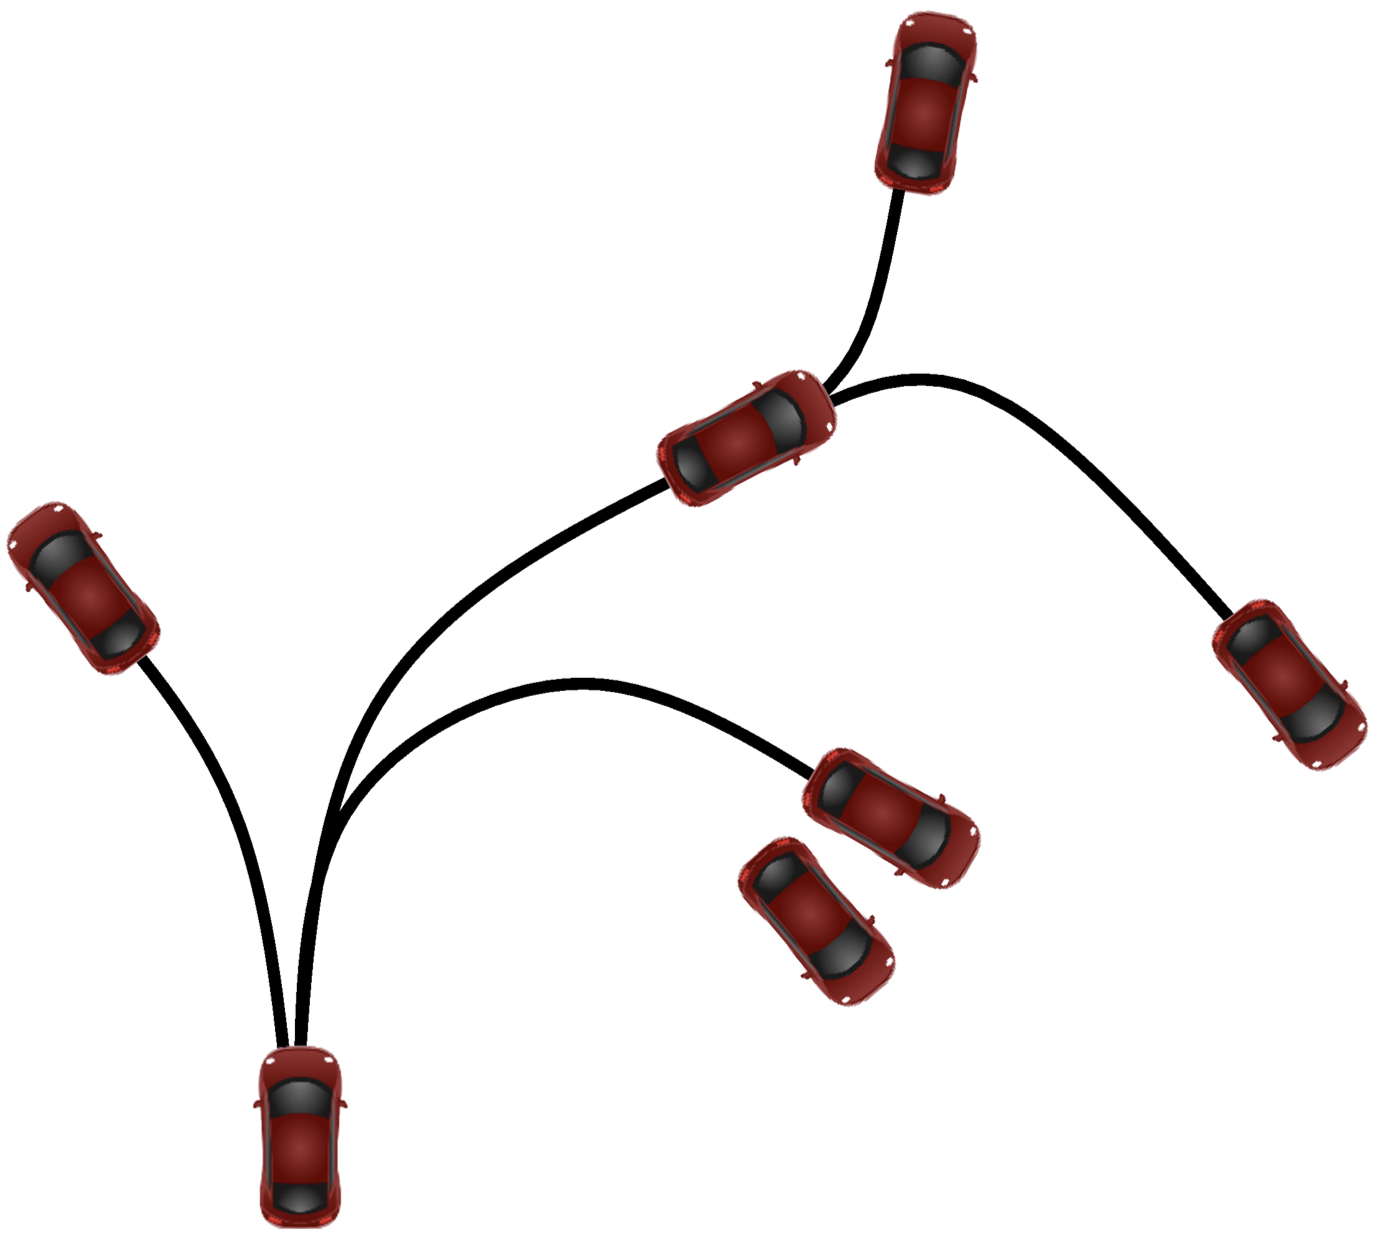
\includegraphics[width=0.5\columnwidth]{Kinodynamic_RRT.jpg}
\end{center}

\subsubsection{RRT*}
Since RRT (and also PRM) are not optimal, we have to ”re-wire” the graph structure to gain optimality.\\
Procedure: For each new sample $q_n$, check its $\log n$ neighborhood and if there are better paths from $q_{start}$ to $q_n$, pick that path.\\
This is an asymptotically optimal sampling based algorithm, because as the number of samples goes to infinity, an optimal path from $q_{start}$ to $q_{goal}$ is obtained.

\section{Probabilistic Robotics}
\subsection{Kalman Filter}
The basic idea of a Kalman filter is that you interpret your robots state as a normal (gaussian) distribution with mean and variance.
Besides the estimate for the state $x$ you also have some estimate for the uncertainty in your value for $x$ that is represented through a normal distribution and its variance / covariance matrix $P$.
You also model your sensors with white noise (gaussian, zero-mean).\\

\textit{\textbf{Explanantion from the internet:}}
A Kalman filter is an optimal estimator i.e. infers parameters of interest
from indirect, inaccurate and uncertain observations.
It is recursive so that new measurements can be processed as they arrive .
If the noise is Gaussian the Kalman filter is optimal, i.e. it minimizes the mean square error of the estimated parameters.\\

\textit{\textbf{Requirements for optimality:}}
\begin{itemize}
	\item Linear system and measurement model
	\item Gaussian and zero-mean measurement and process noise
\end{itemize}

Illustrative:
The more certain the initial estimate is, the higher and narrower the peak.
The greater the noise (amount of error), the faster the peak spreads.\par

Kalman Gain:
\begin{itemize}
	\item $K_k=0$: $R \rightarrow \infty$ or $P_K^- = 0$, i.e. trust in measurement is very low or trust in model is very high.
	\item $K_k=1$: $R = 0$ or $P_K^- \rightarrow \infty$, i.e. trust in measurement is very high or trust in model is very low.
\end{itemize}

\paragraph{Prediction step}
\begin{align*}
	&\text{Mean} && \hat{x}_{k+1}^- = A \hat{x}_{k} + B u_k  \\
	&\text{Covariance } \textcolor{gray}{\sigma_3^2 = \sigma_1^2 + \sigma_2^2} && P_{k+1}^- = A P_k A^\top + Q 
\end{align*}

\paragraph{Update step}
\begin{align*}
	&\text{Kalman Gain} && K_k = P_k^- H^\top (H P_k^- H^\top + R)^{-1} \\
	&\text{Mean} && \hat{x}_k = \hat{x}_k^- + K_k (z_k - H \hat{x}_k^-) \\
	&\text{Covariance } \textcolor{gray}{\frac{1}{\sigma_3^2} = \frac{1}{\sigma_1^2} + \frac{1}{\sigma_2^2}} && P_k = (I - K_k H) P_k^-
\end{align*}
\textbf{with}\\
\vspace{5mm}
\begin{tabular}{ll}
	\\[-1em]
	$\hat{x} \in \mathbb{R}^N$ & state estimate mean \\
	$\hat{x}^- \in \mathbb{R}^N$ & predicted state estimate mean \\
	$A \in \mathbb{R}^{N \times N}$ & state-transition model \\
	$u  \in \mathbb{R}^M$ & control input \\
	$B \in \mathbb{R}^{N \times M}$ & control-input model \\
	$P \in \mathbb{R}^{N \times N}$ & state covariance matrix \\
	$Q  \in \mathbb{R}^{N \times N}$ & process noise covariance  matrix \\
	$K \in \mathbb{R}^{N \times Z}$ & Kalman gain \\
	$R \in \mathbb{R}^{Z \times Z}$ & measurement noise covariance matrix \\
	$z \in \mathbb{R}^Z$ & measurement \\
	$H \in \mathbb{R}^{Z \times N}$ & observation model / measurement matrix
\end{tabular}

\subsubsection{Observability}
\begin{align*}
O = \begin{bmatrix} H \\ HA^1 \\ \vdots  \\ HA^{n-1} \end{bmatrix}
\end{align*}
The system is observable if $\text{rank}(O) = n$ (i.e. $n$ linearly independent rows).
$n$ is the dimension of the state vector $x$.

\subsubsection{Difficulties}
\begin{itemize}
	\item Presence of the unknown and unmeasurable noise vectors $v(k)$ (observation noise) and $w(k)$ (process noise / model error).
	\item The state in general can not be directly observed from the outputs, $H$ may not be invertible.
\end{itemize}

\subsection{Extended Kalman Filter}
The (first order) EKF allows to use non-linear system models for Kalman Filtering and is a sub-optimal extension of the original KF algorithm.
The EKF adapts techniques from calculus, namely multivariate Taylor Series expansions, to linearize the functions $f$ and $h$ around a working point (use the means). 

\paragraph{Prediction step}
\begin{align*}
	%&\text{Working points} && A = A\Bigr|_{x_k=\hat{x}_{k}}, \ W = W\Bigr|_{x_k=\hat{x}_{k}} \\
	&\text{Mean} && \hat{x}_{k+1}^- = f(\hat{x}_k, u_k, 0)  \\
	&\text{Covariance } && P_{k+1}^- = A P_k A^\top + W Q W^\top 
\end{align*}

\paragraph{Update step}
\begin{align*}
	%&\text{Working points} && H = H\Bigr|_{x_k=\hat{x}_{k}^-}, \ V = V\Bigr|_{x_k=\hat{x}_{k}^-} \\
	&\text{Kalman Gain} && K_k = P_k^- H^\top (H P_k^- H^\top + V R V^\top)^{-1} \\
	&\text{Mean} && \hat{x}_k = \hat{x}_k^- + K_k (z_k - h(\hat{x}_k^-, 0)) \\
	&\text{Covariance }  && P_k = (I - K_k H) P_k^-
\end{align*}
\textbf{with}\\
\vspace{5mm}
\begin{tabular}{ll}
	\\[-1em]
	$x_{k+1} = f(x_k, u_k, w_k) \in \mathbb{R}^{N}$ & state transfer function \\
	\\[-1em]
	$w_k \in \mathbb{R}^N$ & process noise \\
	\\[-1em]
	$A = \frac{\partial f}{\partial x_k} \in \mathbb{R}^{N \times N}$ & Jacobian of $f$ with respect to $x_k$ \\
	\\[-1em]
	$W = \frac{\partial f}{\partial w_k} \in \mathbb{R}^{N \times N}$ & Jacobian of $f$ with respect to $w_k$ \\
	\\[-0.3em]
	\hline
	\\[-0.3em]
	$z_k = h(x_k, v_k) \in \mathbb{R}^{Z}$ & measurement function \\
	\\[-1em]
	$v_k  \in \mathbb{R}^{Z}$ & measurement noise \\
	\\[-1em]
	$H = \frac{\partial h}{\partial x_k} \in \mathbb{R}^{Z \times N}$ & Jacobian of $h$ with respect to $x_k$ \\
	\\[-1em]
	$V = \frac{\partial h}{\partial v_k} \in \mathbb{R}^{Z \times Z}$ & Jacobian of $h$ with respect to $v_k$
\end{tabular}

Missing here: EKF for SLAM

\subsection{Unscented Kalman Filter}
Instead of using first order approximations of the Taylor series (EKF), the unscented filter extends to the second (or higher) order approximations.
EKF may cause significant error for highly nonlinear systems because local linearity assumptions break down when the higher order terms become significant.

The idea of the UKF is to produce several sampling points (Sigma Points) from the current state and noise distributions.
Then, propagating these points through the nonlinear map to get a more accurate estimation of the mean and covariance of the mapping results.

The main assumption here is the unscented transformation, which allows to calculate statistics about a random variable that has undergone a nonlinear transformation by saying that it is easier to approximate a probability distribution than an arbitrary nonlinear function.
The estimates of the mean and covariance are accurate to the second order of the Taylor series expansion of the the nonlinear map.
In this way, it avoids the need to calculate the Jacobian, hence incurs only the similar computation load as the EKF.

\paragraph{Initialization}
\begin{align*}
	&\text{State mean} && \hat{x}_{0} = E(x_0) \\
	&\text{Mean vector} && \hat{x}_{0}^a = \begin{bmatrix}\hat{x}_{0}^\top & 0 & 0 \end{bmatrix}^\top \\
	\intertext{\small Contains mean values of state ($x$), process noise ($v$) and measurement noise ($n$). $x_t^a = [x_t^\top,v_t^\top,n_t^\top]$}
	&\text{Covariance matrix }  && P_{0}^a = \begin{bmatrix}P_{0} & 0 & 0 \\ 0 & Q & 0 \\ 0 & 0 & R\end{bmatrix} 
	\intertext{\small Covariance matrices of state $P_0$, process noise $Q$ and measurement noise $R$.}
\end{align*}

\paragraph{Prediction step}\mbox{}\\
\textit{(a) Computing sigma points}
\begin{flalign*}
	&\text{Sigma points} \qquad \chi_{k-1}^a = \begin{bmatrix}\hat{x}_{k-1}^a & \hat{x}_{k-1}^a \pm \sqrt{(n_x + \lambda) P_{k-1}^a } \end{bmatrix}
\end{flalign*}
\textit{(b) Time update}
\begin{align*}
	&\text{Sigma points} && (\chi_{k}^x)^- = f(\chi_{k-1}^x, \chi_{k-1}^v) \\
	&\text{State mean} && \hat{x}_{k}^- = \sum_{i=0}^{2n_x} W_i^{(m)} (\chi_{i,k}^x)^- \\
	&\text{Covariance} && P_k^- = \sum_{i=0}^{2n_x} W_i^{(c)} \begin{bmatrix} (\chi_{i,k}^x)^- - \hat{x}_{k}^-\end{bmatrix}\begin{bmatrix} (\chi_{i,k}^x)^- - \hat{x}_{k}^-\end{bmatrix}^\top
\end{align*}

\paragraph{Update step}

\begin{align*}
	&\text{Predicted meas.} && Y_k^- = h((\chi_{k}^x)^-, \chi_{k-1}^n) \\
	&\text{Meas. mean} && \hat{y}_{k}^- = \sum_{i=0}^{2n_x} W_i^{(m)} Y_{i,k}^- \\
	&\text{Meas. cov.} && P_{y_k y_k} = \sum_{i=0}^{2n_x} W_i^{(c)} \begin{bmatrix}Y_{i,k}^- - \hat{y}_{k}^-\end{bmatrix} \begin{bmatrix}Y_{i,k}^- - \hat{y}_{k}^-\end{bmatrix}^\top \\
	&\text{Cross cov.} && P_{x_k y_k} = \sum_{i=0}^{2n_x} W_i^{(c)} \begin{bmatrix}\chi_{i,k}^{x-} - \hat{x}_{k}^-\end{bmatrix} \begin{bmatrix}Y_{i,k}^- - \hat{y}_{k}^-\end{bmatrix}^\top \\
	&\text{Kalman Gain} && K_k = P_{x_k y_k} P_{y_k y_k}^{-1} \\
	&\text{State mean} && \hat{x}_k = \hat{x}_k^- + K_k(y_k - \hat{y}_k^-) \\
	&\text{Covariance} && P_k = P_k^- - K_k P_{y_k y_k} K_k^\top
\end{align*}

\paragraph{Notation}
\begin{flalign*}
	&x^a = [x^\top,v^\top,n^\top], \quad \chi^a = [(\chi^x)^\top,(\chi^v)^\top,(\chi^n)^\top]^\top \\
	&n_a = n_x + n_v + n_n: \text{ Dimension of $x$, $v$ and $n$.}\\
	& \lambda: \text{ Composite scaling parameter.}\\
	&W: \text{ Weights}
\end{flalign*}

\paragraph{Weights}
\begin{flalign*}
	&W_{0}^{(m)} = \frac{\lambda}{n_x + \lambda} \\
	&W_{0}^{(c)} = \frac{\lambda}{n_x + \lambda} + (1 - \alpha^2 + \beta) \\
	&W_i^{(m)} = W_i^{(c)} = \frac{\lambda}{2(n_x + \lambda)}, i=1,\dots,2n_x
\end{flalign*}


\subsection{Bayes Filter}

\paragraph{Assumptions:}
\begin{itemize}
	\item Markov property: $P(x_k|x_{k-1},\dots,x_0) = P(x_k|x_{k-1})$
	\item Observation: $P(y_k|x_k,\dots,x_0) = P(y_k|x_k)$
\end{itemize}

\paragraph{Given:}
\begin{itemize}
	\item Measurements: $y_{1:k} = y_1, \dots, y_k$
	\item Control inputs: $u_{0:k-1} = u_0, \dots, u_{k-1}$
	\item Dynamic model (e.g. motion model): $P(x_{k+1}|x_k,u_k)$
	\item Prior probability: $P(x_0)$
	\item Sensor model: $P(y_k|x_k)$
\end{itemize}

\begin{center}
	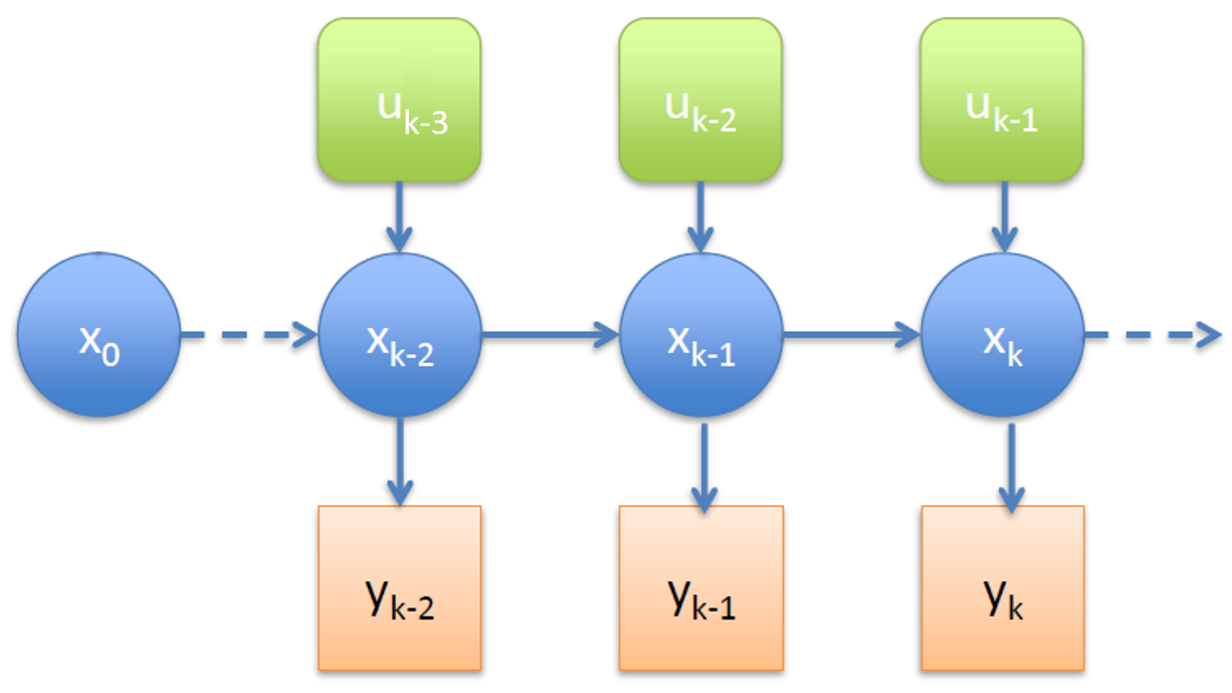
\includegraphics[width=0.7\columnwidth]{bayes_filter.PNG}
\end{center}

\paragraph{Compute:}\mbox{}\\
Most likely state $x$ at time $k$ given commands $u_{0:k-1}$ and measurements $y_{1:k-1}$(posterior distribution)
\begin{flalign*}
	P&(x_k|y_{1:k},u_{0:k-1}) = \frac{P(y_k|x_k,y_{1:k-1},u_{0:k-1}) P(x_k|y_{1:k-1},u_{0:k-1})}{P(y_k|y_{1:k-1},u_{0:k-1})} \\
	&= \eta_k \underbrace{P(y_k|x_k)}_{\text{observation}} \int_{x_{k-1}} \underbrace{P(x_k|u_{k-1},x_{k-1})}_{\text{state prediction}} \underbrace{P(x_{k-1}|y_{1:k-1},u_{0:k-2})}_{\text{recursive instance}}dx_{k-1}
\end{flalign*}

Without measurements, only prediction:
\begin{equation*}
	P(x_k) = \int_{x_{k-1}} P(x_k|x_{k-1},u_{k-1}) P(x_{k-1}) dx_{k-1}
\end{equation*}


\subsection{Particle Filter}
The state representations of the Bayes and Kalman filter are restricted to probability density or Gaussian functions.
They also cannot model multiple hypotheses in their initial form, for example the uncertainty when a robot could be in one of multiple locations.
(Multi-hypothesis KF could do that, but it's only a combination of multiple KFs).

The particle filter uses a population of randomly initialized particles to track high-likelihood regions of the state space.
The basic procedure is:
\begin{enumerate}
	\item If no initial distribution is given, start with a uniform sample distribution.
	\item Apply motion model to particles by sampling from the corresponding distribution. \label{pMM}
	\item After observing the measurement, weight each particle by its likelihood for the observation.
	\item Resampling: Generate a new set of samples by weighted random selection from the current set of particles.
	\item Repeat from \ref{pMM}.
\end{enumerate}
At any time, the distribution is represented by the weighted set of particles.

\paragraph{Particle Deprivation:} There are not particles in the vicinity of the correct state.
\begin{itemize}
	\item Occurs as the result of the variance in random sampling.
	An unlucky series of random numbers can wipe out all particles near the true state.
	This has non-zero probability to happen at each time $\rightarrow$ will happen eventually.
	\item Popular solution: Add a small number of randomly generated particles when resampling.
\end{itemize}

\paragraph{Problem with Resampling:}
Resampling induces loss of diversity.
The variance of the particles decreases, the variance of the particle set as an estimator of the true belief increases.
\begin{itemize}
	\item Solution 1: Resample only when effective sample size is low.
	\item Solution 2: Low-variance-sampling.
\end{itemize}


\end{multicols*}
\end{document}